\documentclass[a4paper, 12pt]{article}%тип документа

%отступы
\usepackage[left=0.6cm,right=1cm,top=2cm,bottom=3cm,bindingoffset=0cm]{geometry}
\setlength{\parindent}{5ex}

%Русский язык
\usepackage[T2A]{fontenc} %кодировка
\usepackage[utf8]{inputenc} %кодировка исходного кода
\usepackage[english,russian]{babel} %локализация и переносы

%Вставка картинок
\usepackage{graphicx}
\graphicspath{{pictures/}}
\DeclareGraphicsExtensions{.pdf,.png,.jpg}

%Графики
\usepackage{pgfplots}
\pgfplotsset{compat=1.9}

%Математика
\usepackage{amsmath, amsfonts, amssymb, amsthm, mathtools}

%Таблицы
\usepackage{longtable} 
\usepackage{float}

%Римские цифры
\newcommand{\RomanNumeralCaps}[1]{\uppercase\expandafter{\romannumeral#1}}

\usepackage{multirow}


\begin{document}
	\begin{titlepage}
		\begin{center}
			\textsc{Федеральное государственное автономное образовательное учреждение высшего образования«Московский физико-технический институт (национальный исследовательский университет)»\\[5mm]
			}
			
			\vfill
			
			\textbf{Отчёт по лабораторной работы 4.4.3\\[3mm]
				ИЗУЧЕНИЕ ПРИЗМЫ С ПОМОЩЬЮ
				ГОНИОМЕТРА
				\\[50mm]
			}
			
		\end{center}
		
		\hfill
		\begin{minipage}{.5\textwidth}
			Выполнил студент:\\[2mm]
			Сериков Василий Романович\\[2mm]
			группа: Б03-102\\[5mm]
			
		\end{minipage}
		\vfill
		\begin{center}
			Москва, 2023 г.
		\end{center}
		
	\end{titlepage}
	
	\newpage
	\textbf{Аннотация}\\
	
	
	\textbf{Цель работы: }\\
	Знакомство с работой гониометра и определение спектральных характеристик амплитудной или фазовой решётки (эшелета).\\
	
	\textbf{В работе используются: }\\
	Ртутная лампа, гониометр, амплитудная
	и фазовая дифракционные решётки, плоскопараллельная стеклянная
	пластинка, призменный уголковый отражатель, щель с микрометрическим винтом.\\
	
	\textbf{Теоретические сведения: } \\
	
	Гониометр служит для точного измерения углов и находит широкое применение в оптических лабораториях. С помощью гониометра можно определять показатели преломления и преломляющие углы призм и кристаллов, исследовать параметры дифракционных решёток, измерять длины волн спектральных линий и т. д. В настоящей работе прибор применяется для исследования дисперсии стеклянных призм --- зависимости показателя преломления от длины волны.
	
	\begin{figure}[H]
		\begin{center}
			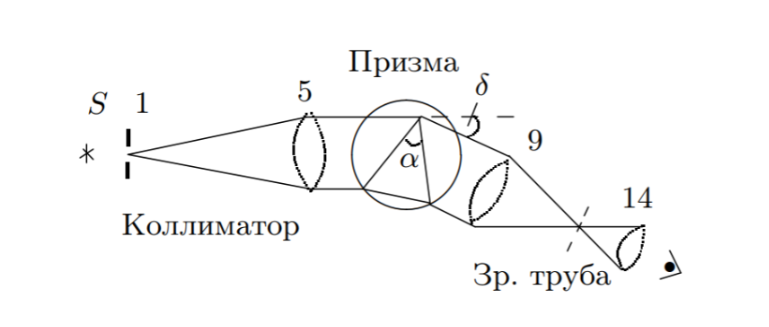
\includegraphics[width = 0.85\textwidth]{1.png}
			\caption{Оптическая схема эксперимента}
		\end{center}
	\end{figure}

	Показатель преломления материала призмы удобно определять по углу наименьшего отклонения. Известно, что минимальное отклонение луча, преломленного призмой, от направления луча, падающего на призму, получается при симметричном ходе луча (в призме луч идёт перпендикулярно биссектрисе преломляющего угла). Угол минимального отклонения $\delta$, преломляющий угол $\alpha$ (угол при вершине призмы на рис. 1) и показатель преломления $n$ связаны между собой соотношением
	\begin{equation}
		n=\dfrac{\sin\dfrac{\alpha+\delta}{2}}{\sin\dfrac{\alpha}{2}}.
	\end{equation}
	Измерив с помощью гониометра преломляющий угол призмы и углы наименьшего отклонения для света разных длин волн, можно рассчитать величину $n$ и построить дисперсионную кривую --- график зависимости $n(\lambda)$. 
	
	По дисперсионной кривой могут быть определены такие важные характеристики оптических стёкол, как средняя дисперсия
	\begin{equation}
		D = n_F - n_C
	\end{equation}
	и коэффициент дисперсии $\nu$ (число Аббе):
	\begin{equation}
		\nu = \dfrac{n_D - 1}{n_F - n_C},
	\end{equation}
	где $n_D, n_F$ и $n_C$ --- показатели преломления для $\lambda_D = 589{,}3$ нм (среднее значение длин волн жёлтого дублета натрия), $\lambda_F = 486{,}1$ нм (голубая линия водорода), $\lambda_C = 656{,}3$ нм (красная линия водорода).
	
	По наклону дисперсионной кривой можно оценить разрешающую
	способность призмы
	\begin{equation}
		R = \dfrac{\lambda}{\delta\lambda} = b\dfrac{dn}{d\lambda}.
	\end{equation}
	Здесь $\delta\lambda$ --- минимальный интервал длин волн, разрешаемый по критерию Релея, $b$ --- размер основания призмы, если вся рабочая грань призмы освещена параллельным пучком.\\
	
	\textbf{Ход работы и обработка результатов.}\\
	
	
		
	\RomanNumeralCaps 1 \textit{Измерение преломляющего угла:}\\

	 Для измерения преломляющего угла $\gamma$ призмы установим трубу перпендикулярно одной из её отражающих граней и снимем отсчёт по лимбу. Затем, не трогая призму	и столик, повернем алидаду с трубой вокруг преломляющего угла призмы и проведем ту же операцию для другой рабочей грани. По углу поворота трубы рассчитаем преломляющий угол призмы.
	
	\begin{longtable}{|c|c|c|c|}
		\hline
		$\alpha_1$ & $\alpha_2$ & a, мм & $\gamma$ \\ \hline
		$186^\circ 50'37''$ & $303^\circ 49'53''$ & 71,5 & 	$58^\circ 29'58''$\\ \hline
		\caption{Таблица с данными расчета угла преломления призмы. $\sigma = 5''$ -- погрешность измерения углов}
	\end{longtable}

	\RomanNumeralCaps 2 \textit{Минимальный угол отклонения: } \\
	
	Для определения минимального угла отклонения $\delta$ необходимо поворачивать столик и, наблюдая за перемещением спектра, найти положение столика с призмой, соответствующее минимальному отклонению преломлённого луча от направления падающего луча.
	Полученные углы для спектра занесем в таблицу 2.
	
	\begin{longtable}{|c|c|c|c|c|c|c|c|c|}
		\hline
		№ & $K_1$ & $K_2$ & 1 & 2 & 3 & 4 & 5 & 6 \\ \hline
		$\lambda,$ нм & 690,7 & 623,4 & 579,1 & 577,0 & 546,1 & 491,6 & 435,8 & 404,7 \\ \hline
		Цвет &красн.&красн.& желт. & желт. & зелен. & голуб. & синий & фиолет. \\ \hline
		Яркость & 4 & 4&10 & 8 & 10 & 4 & 4 & 3 \\ \hline
		$\delta$ & 	$128^\circ 53'42''$ & $128^\circ 26'59''$ & $128^\circ 3'49''$ & $128^\circ 2'11''$ & $127^\circ 42'19''$ & $126^\circ 55'3''$ & $125^\circ 43'43''$ & $124^\circ 45'45''$ \\ \hline
		\caption{Характеристики спектра ртутной лампы ДРШ--250}
	\end{longtable}
	
	\newpage
	
	\RomanNumeralCaps 3 \textit{Обработка полученных результатов: } \\
	\begin{enumerate}
	\item Рассчитаем показатель преломления $n(\gamma,\delta)$ по формуле (1),считая $\delta = 180^\circ - \delta$ . Построим дисперсионную кривую $n(\lambda)$
	
	\begin{longtable}{|c|c|c|c|c|c|c|c|c|}
		\hline
		 &$K_1$ & $K_2$ & 1 & 2 & 3 & 4 & 5 & 6 \\ \hline
		n &1,672 & 1,676 & 1,681 & 1,681 & 1,684 & 1,692 & 1,704 & 1,713 \\ \hline
		\caption{Показатели преломления на различных спектральных составляющих. $\sigma_n = 0,002$}
	\end{longtable}

	\begin{figure}[H]
		\center{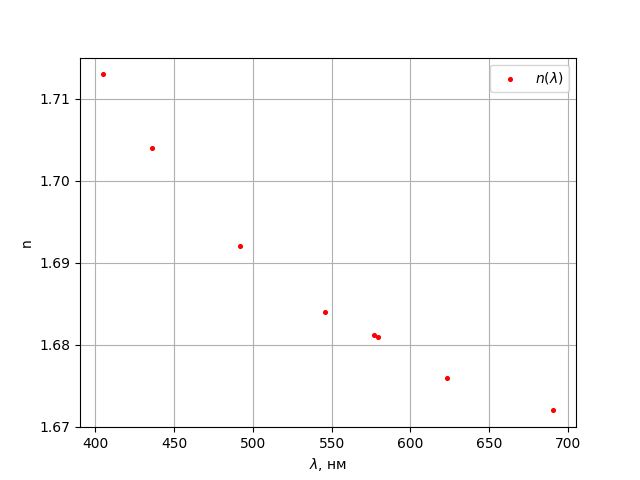
\includegraphics[scale=0.9]{n(lambda).png}}
		\caption{График зависимости $n(\lambda)$.}
	\end{figure}

	\newpage
	
	\item Определим по графику	$n_D$, $n_F$, $n_C$ и $dn/d\lambda$ и рассчитаем среднюю дисперсию стекла по формуле (2), рассчитаем число Аббе по формуле (3) и рассчитаем максимальную разрешающую
	способность R призмы по формуле (4).
	
	\begin{longtable}{|c|c|c|c|c|c|c|}
		\hline
		$n_D$ & $n_F$ & $n_C$ & D & $\nu$ & $dn/d\lambda$ & R  \\ \hline
		1,679$\pm 0,002$ & 1,693$\pm 0,002$ & 1,674$\pm 0,002$ & 0,019$\pm 0,004$ & 35,71$\pm 0,04$& (28,94$\pm 0,03$)$\cdot 10^4$ & (20,7$\pm 0,3$)$\cdot 10^3$\\ \hline
		\caption{Значения параметров стекла призмы}
	\end{longtable}
	
	\end{enumerate}
	
	\textbf{Обсуждение результатов и выводы: }\\
	
	В данной работе мы познакомились с гониометром, исследовали дисперсии стеклянной призмы и определили характеристики призмы как
	спектрального прибора.
	Определили угол преломления призмы $\gamma =  58^\circ 29'58''\pm 0^\circ 0'5''$.
	Определили среднюю дисперсию, коэффициент Аббе и $n_D$, $n_F$, $n_C$, $\nu$ по данным значениям можно сказать, что стекло сорта БФ-28 - баритовый флинт ($n_D$ = 1,6641, $n_F$ - $n_C$ = 0,01874, $\nu$ = 35,4)
	
	
	
	\end{document}